%!TEX root = ../problems.tex
\begin{task}
	Найти спектр сигнала, изображенного на рисунке. Построить график $|S(w)|$.
\end{task}
\begin{figure}[h!]
	\centering
	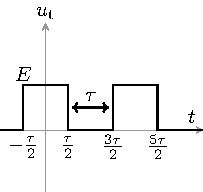
\includegraphics[width = .4\linewidth]{ris/task9_input.pdf}
	\caption{}
	\label{fig:9}
\end{figure}

\begin{proof}[\rm{\textbf{Решение}}]
	В силу линейности преобразования Фурье, и свойства смещения двух прямоугольных импульсов $ U(t) = u_1(t)+u_2(t)$,
	получим:
	$$ \widehat{S(w)} = S_1(w) +S_2(w) = S(w)(1+e^{-2\cdot iw\tau}) $$
	,где $ S(w) = A\tau\frac{\sin{\frac{w\tau}{2}}}{\frac{w\tau}{2}} = A\tau ~ sinc(\frac{w\tau}{2}) $ - спектр прямоугольного импульса.
	
	Тогда, свернув сумму экспонент по формуле Эйлера, получим:
	$$ \widehat{S(w)} = A\tau~sinc(\frac{w\tau}{2}) \cdot e^{-iw\tau}\frac22(e^{-iw\tau}+e^{iw\tau}) =
	2A\tau~sinc(\frac{w\tau}{2}) \cdot e^{-iw\tau} \cos{w\tau} $$

	$$ |S(w)| = 2A\tau~ |~sinc~(\frac{w\tau}{2})  \cos{w\tau}~|  $$
	\begin{figure}[h!]
		\centering
		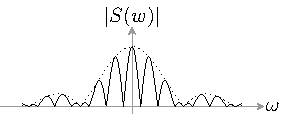
\includegraphics[width = .6\linewidth]{ris/task9_out.pdf}
		\caption{}
		\label{fig:9.1}
	\end{figure}

\end{proof}